\section{Context and beam physics}
% Original presentation frame 2
\begin{frame}[t,shrink=5]{The presentation separates established physics from the work developed in this work}
\begin{columns}[T,onlytextwidth]
\begin{column}{0.49\textwidth}
\begin{block}{Scientific context}
\begin{enumerate}
\item FCC-ee HEB and collective instabilities.
\item Distribution-level beam dynamics.
\item Simulation cost and prior surrogate methods.
\end{enumerate}
\end{block}

\end{column}
\begin{column}{0.49\textwidth}
\begin{block}{Main contributions}
\begin{enumerate}
\item Reproducible Xsuite/PyColleff datasets and projected 6D representation.
\item FNO, CVAE, Transformer, local-window Transformer and GNO surrogates.
\item Common endpoint comparison: distributions, physical statistics and runtime.
\item Conditional latent-uncertainty study, limitations and next validation steps.
\end{enumerate}
\end{block}

\end{column}
\end{columns}

\sources{Preliminary FCC-ee HEB results: \parencite{ghribi2026updates}.}

\end{frame}

% Original presentation frame 3
\begin{frame}[t,shrink=5]{The FCC-ee HEB must preserve beam quality while ramping through a 90.7 km accelerator complex}
\begin{columns}[T,onlytextwidth]
\begin{column}{0.49\textwidth}
\begin{block}{Role in the injection chain}
\begin{itemize}
\item FCC-ee is the leading flagship project in CERN's post-LHC programme.
\item The HEB follows the high-energy injector stage and shares the collider-tunnel infrastructure.
\item It ramps from about 20 GeV to the collider injection energies 45.6--182.5 GeV.
\item Its task is to deliver the required intensity and phase-space quality for top-up injection.
\end{itemize}
\end{block}
\begin{block}{Machine complexity}
{\scriptsize The exact lattice-element count is not fixed. The HEB full lattice in the present work contains about 17,000 elements. The lattice is a simplified version of the FCC-ee HEB lattice v24.1.\par}
\end{block}

\end{column}
\begin{column}{0.49\textwidth}
\begin{center}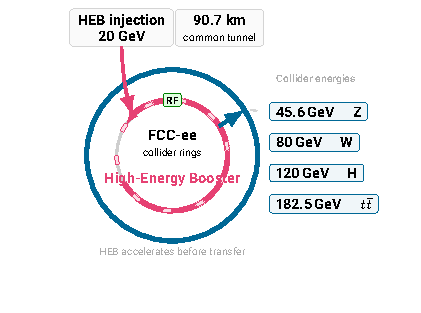
\includegraphics[width=\linewidth]{fcc_ee_heb_injection_chain.pdf}\end{center}
\end{column}
\end{columns}

\sources{\parencite{fcc2025feasibility,fcc2026lattice,ghribi2026collective,zimmermann2024fcc}.}

\end{frame}

% Original presentation frame 4
\begin{frame}[t,shrink=5]{Collective forces make beam transport a nonlinear operator on the distribution}
\begin{columns}[T,onlytextwidth]
\begin{column}{0.49\textwidth}
\begin{block}{Beam-distribution evolution}
\[\rho_s(\xi)\longmapsto\rho_{s+\Delta s}(\xi),\quad\xi=(x,p_x,y,p_y,\zeta,\delta).\]
The force is separated into physical pieces:
\[\frac{\partial\rho_s}{\partial s}+\nabla_\xi\!\cdot[\rho_s(F_{\rm ext}+F_{\rm coll}[\rho_s]+F_{\rm rad})]=\frac12\nabla_\xi\nabla_\xi:(D_{\rm rad}\rho_s).\]
\end{block}
\begin{alertblock}{Operator-learning target}
The validated object is the endpoint map\[\mathcal G_\mu:\rho_{\rm in}\longrightarrow\rho_{\rm out}.\]
\end{alertblock}

\end{column}
\begin{column}{0.49\textwidth}
\begin{block}{First-order operator splitting used as the conceptual model}
\[\rho_{j+1}\approx e^{\Delta s\mathcal D_j}e^{\Delta s\mathcal C_j[\rho_j]}(M_{j,\mu_j})_{\#}\rho_j.\]
\scriptsize external lattice $\to$ collective kick $\to$ radiation / diffusion
\end{block}
\begin{alertblock}{Key learning objective}
The model is focused in the nonlinear collective operator, which is the only piece that depends on the distribution itself.
\end{alertblock}

\end{column}
\end{columns}

\sources{\parencite{metral2021wake,wiedemann2015vlasov}.}

\end{frame}

% Original presentation frame 5
\begin{frame}[t,shrink=5]{High-particle tracking is cheap once, but repeated scans turn it into a CPU-budget problem}
\begin{columns}[T,onlytextwidth]
\begin{column}{0.45\textwidth}
\begin{center}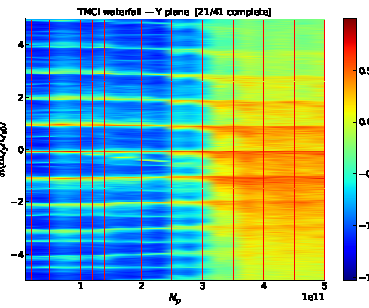
\includegraphics[width=\linewidth]{tmci_y_plane_waterfall.pdf}\end{center}
\end{column}
\begin{column}{0.53\textwidth}
\begin{block}{Timing retained}
\begin{center}\begin{adjustbox}{max width=\linewidth}
\begin{tabular}{lrrr}\toprule Stage & $t_{\rm sample}$ & \multicolumn{2}{c}{CPU-core h}\\ & & 2048 & $10^5$\\\midrule
Xsuite, $10^6$ particles & 1.41 s & 0.807 & 39.2\\
PyColleff, $N_\zeta=2048$ & 2.72 s & 1.547 & 75.6\\
6D histograms & 2.32 ms & $1.32\times10^{-3}$ & $6.44\times10^{-2}$\\\bottomrule\end{tabular}
\end{adjustbox}\end{center}
\end{block}
{\scriptsize CC-IN2P3 \texttt{gpu\_v100} host: $4\times$ NVIDIA Tesla V100 PCIe (32 GB HBM2), 192 GB RAM and two Intel Xeon Silver 4114/4214R CPUs, 20--24 cores per node. One fully allocated node-hour therefore represents 20--24 CPU-core h.\par}\begin{block}{Simulation record required for this scan}
{\scriptsize The data has been simulated for 1000 turns, 20 GeV, using the full longitudinal wake/impedance budget, Z mode. IBS, space charge and synchrotron radiation disabled. All has been simulated at CC-IN2P3 in CPU mode.\par}
\end{block}

\end{column}
\end{columns}

\sources{\parencite{iadarola2023xsuite,xsuite2026documentation,ccin2p3slurm,rigaud2021gpu,fcc2026lattice}.}

\end{frame}

